\documentclass[aspectratio=169]{beamer}
\usetheme{default}
\usecolortheme{default}

\usepackage{graphicx}
\usepackage{tikz}
\usepackage{listings}
\usepackage{xcolor}

\setbeamercolor{structure}{fg=black}
\setbeamercolor{frametitle}{bg=white,fg=black}
\setbeamertemplate{navigation symbols}{}
\setbeamertemplate{footline}{}
\setbeamertemplate{headline}{}

\title{AI-Powered Educational Management System}
\subtitle{A Comprehensive Full-Stack Solution with Role-Based Dashboards}
\date{\today}

\begin{document}

% Slide 1: Title Slide
\begin{frame}
\begin{center}
\includegraphics[width=2.5cm]{adypu-logo.png}
\end{center}
\vspace{0.3em}
\begin{center}
{\Large \textbf{AI-Powered Educational Management System}}\\
{\large A Comprehensive Full-Stack Solution with Role-Based Dashboards}
\end{center}
\vspace{0.5em}
\begin{columns}
\begin{column}{0.55\textwidth}
\small
\textbf{Name:} Priyanshu Kumar Sharma \\
\textbf{Program:} BTech IT (CTIS) \\
\textbf{URN No:} 2022-B-17102004A \\
\textbf{Project Id:} Your Project ID \\
\textbf{Team Members:} \\
\quad • Vaishnavi Jadhav \\
\quad • Vaibhav Gulage
\end{column}
\begin{column}{0.45\textwidth}
\small
\raggedleft
\textbf{Guide Name:} \\
Prof. Prini Rastogi
\end{column}
\end{columns}
\end{frame}

% Slide 2: Table of Contents
\begin{frame}{Table of Contents}
\begin{itemize}
\item Introduction
\item Problem Statement
\item Literature Review
\item Research Methodology
\item System Architecture
\item Key Features
\item AI Integration
\item Implementation
\item Demo
\item Deployment
\item Future Scope
\item References
\item Conclusion
\end{itemize}
\end{frame}

% Slide 3: Introduction
\begin{frame}{Introduction}
\begin{itemize}
\item \textbf{Project:} AI-Powered Educational Management System
\item \textbf{Type:} Full-Stack Web Application
\item \textbf{Target Users:} Administrators, Teachers, Students
\item \textbf{Key Innovation:} AI integration with role-based dashboards
\item \textbf{Languages:} Bilingual support (English/Hindi)
\end{itemize}

\vspace{1em}
\textbf{Mission:} Revolutionizing education through intelligent technology and seamless user experience
\end{frame}

% Slide 4: Problem Statement
\begin{frame}{Problem Statement}
\begin{itemize}
\item Traditional educational systems lack digital integration
\item Limited personalized learning support for students
\item Inefficient communication between teachers and students
\item Manual administrative processes are time-consuming
\item Language barriers in diverse educational environments
\item Need for real-time collaboration and assessment tools
\end{itemize}

\vspace{1em}
\textbf{Solution:} Comprehensive AI-powered platform addressing all stakeholder needs
\end{frame}

% Slide 5: Literature Review
\begin{frame}{Literature Review}
\textbf{Existing Systems Analysis:}
\begin{itemize}
\item \textbf{Moodle LMS [1]:} Open-source LMS, limited AI integration
\item \textbf{Google Classroom [2]:} Cloud-based platform, lacks AI tutoring
\item \textbf{Khan Academy [3]:} Personalized dashboards, basic adaptive learning
\item \textbf{Blackboard Learn [4]:} Enterprise LMS, limited multilingual support
\item \textbf{Coursera [5]:} MOOC platform, focuses on higher education
\end{itemize}

\textbf{Research Gap:}
\begin{itemize}
\item Comprehensive AI integration across all user roles
\item Real-time bilingual support with live translation
\item Unified platform combining LMS, AI tutoring, and development tools
\end{itemize}
\end{frame}

% Slide 6: Research Methodology
\begin{frame}{Research Methodology}
\textbf{Development Approach:}
\begin{itemize}
\item \textbf{Agile Methodology:} Iterative development with continuous feedback
\item \textbf{Full-Stack Development:} Integrated frontend and backend
\item \textbf{API-First Design:} RESTful APIs for modular architecture
\item \textbf{Component-Based Architecture:} Reusable React components
\end{itemize}

\textbf{AI Integration Algorithm:}
\begin{itemize}
\item User query preprocessing and context analysis
\item Intent classification using NLP models
\item OpenAI API integration for intelligent responses
\item Real-time translation using Google Translate API
\item Response optimization and delivery
\end{itemize}
\end{frame}

% Slide 7: System Architecture
\begin{frame}{System Architecture}
\begin{center}
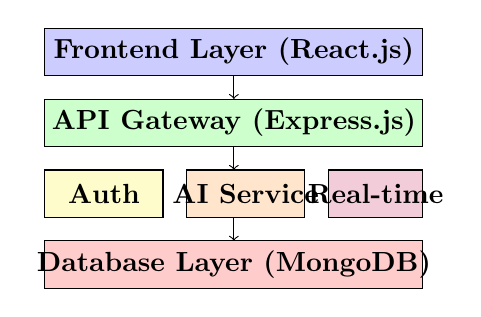
\begin{tikzpicture}[scale=0.6]
\draw[fill=blue!20] (0,4) rectangle (8,5);
\node at (4,4.5) {\textbf{Frontend Layer (React.js)}};

\draw[fill=green!20] (0,2.5) rectangle (8,3.5);
\node at (4,3) {\textbf{API Gateway (Express.js)}};

\draw[fill=yellow!20] (0,1) rectangle (2.5,2);
\node at (1.25,1.5) {\textbf{Auth}};

\draw[fill=orange!20] (3,1) rectangle (5.5,2);
\node at (4.25,1.5) {\textbf{AI Service}};

\draw[fill=purple!20] (6,1) rectangle (8,2);
\node at (7,1.5) {\textbf{Real-time}};

\draw[fill=red!20] (0,-0.5) rectangle (8,0.5);
\node at (4,0) {\textbf{Database Layer (MongoDB)}};

\draw[->] (4,4) -- (4,3.5);
\draw[->] (4,2.5) -- (4,2);
\draw[->] (4,1) -- (4,0.5);
\end{tikzpicture}
\end{center}

\textbf{Tech Stack:}
\begin{itemize}
\item \textbf{Frontend:} React.js, Tailwind CSS, Socket.io Client
\item \textbf{Backend:} Node.js, Express.js, MongoDB Atlas
\item \textbf{AI APIs:} OpenAI, Google Translate, TensorFlow.js
\end{itemize}
\end{frame}

% Slide 8: Key Features - Admin
\begin{frame}{Key Features - Admin Dashboard}
\begin{itemize}
\item \textbf{Teacher Management}
  \begin{itemize}
  \item Add, edit, delete teachers
  \item Assign subjects and classes
  \end{itemize}
\item \textbf{Student Management}
  \begin{itemize}
  \item Complete student lifecycle management
  \item Enrollment and performance tracking
  \end{itemize}
\item \textbf{Analytics Dashboard}
  \begin{itemize}
  \item Real-time statistics and metrics
  \item Usage analytics and reports
  \end{itemize}
\item \textbf{System Logs \& Reports}
  \begin{itemize}
  \item Activity tracking and audit trails
  \end{itemize}
\end{itemize}
\end{frame}

% Slide 9: Key Features - Teacher & Student
\begin{frame}{Key Features - Teacher \& Student}
\textbf{Teacher Portal:}
\begin{itemize}
\item \textbf{Virtual Classroom:} Live video sessions with WebRTC
\item \textbf{Quiz Management:} Create custom quizzes with auto-grading
\item \textbf{Class Management:} Student roster and attendance tracking
\end{itemize}

\textbf{Student Hub:}
\begin{itemize}
\item \textbf{Virtual Classes:} Join live sessions with real-time translation
\item \textbf{AI Tutor:} ChatGPT-powered 24/7 academic assistance
\item \textbf{Virtual Code Editor:} Online coding environment
\item \textbf{Materials \& Assessments:} Access notes, quizzes, and exams
\end{itemize}
\end{frame}

% Slide 10: AI Integration
\begin{frame}{AI Integration}
\begin{center}
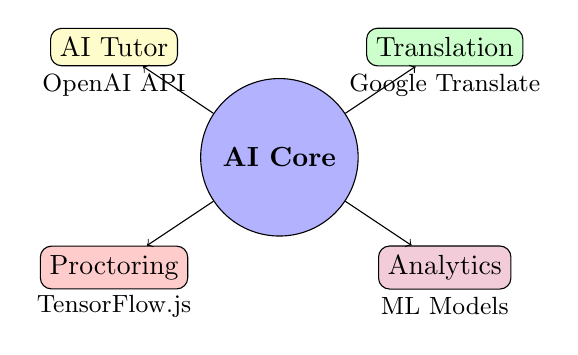
\begin{tikzpicture}[scale=0.7]
\node[draw,circle,fill=blue!30,minimum size=2cm] (ai) at (0,0) {\textbf{AI Core}};

\node[draw,rounded corners,fill=yellow!20] (tutor) at (-3,2) {AI Tutor};
\node[draw,rounded corners,fill=green!20] (translate) at (3,2) {Translation};
\node[draw,rounded corners,fill=red!20] (proctor) at (-3,-2) {Proctoring};
\node[draw,rounded corners,fill=purple!20] (analytics) at (3,-2) {Analytics};

\draw[->] (ai) -- (tutor);
\draw[->] (ai) -- (translate);
\draw[->] (ai) -- (proctor);
\draw[->] (ai) -- (analytics);

\node at (-3,1.3) {\small OpenAI API};
\node at (3,1.3) {\small Google Translate};
\node at (-3,-2.7) {\small TensorFlow.js};
\node at (3,-2.7) {\small ML Models};
\end{tikzpicture}
\end{center}

\textbf{AI Components [6-8]:}
\begin{itemize}
\item \textbf{AI Tutor:} ChatGPT-powered intelligent assistance
\item \textbf{Translation:} Real-time multilingual support
\item \textbf{Proctoring:} AI-based examination monitoring
\item \textbf{Analytics:} Machine learning-driven insights
\end{itemize}
\end{frame}

% Slide 11: Implementation
\begin{frame}{Implementation}
\textbf{Database Schema:}
\begin{columns}
\begin{column}{0.5\textwidth}
\textbf{User Model:}
\begin{itemize}
\item username, password
\item role (admin/teacher/student)
\item fullName, email
\item isActive, refreshToken
\end{itemize}

\textbf{Teacher Model:}
\begin{itemize}
\item userId (reference)
\item qualifications
\item subjects, assignedClasses
\end{itemize}
\end{column}
\begin{column}{0.5\textwidth}
\textbf{Student Model:}
\begin{itemize}
\item userId (reference)
\item enrollNo, standard
\item parentsContact, address
\end{itemize}

\textbf{Additional Models:}
\begin{itemize}
\item Quiz, Classroom
\item Authentication tokens
\item Activity logs
\end{itemize}
\end{column}
\end{columns}

\textbf{Authentication:} JWT-based with role-based access control [9]
\end{frame}

% Slide 12: Demo
\begin{frame}{Demo \& Testing}
\begin{center}
\textbf{Demo Credentials:}
\begin{tabular}{|c|c|c|}
\hline
\textbf{Role} & \textbf{Username} & \textbf{Password} \\
\hline
Admin & admin & admin123 \\
\hline
Teacher & teacher1 & teacher123 \\
\hline
Student & student1 & student123 \\
\hline
\end{tabular}
\end{center}

\vspace{1em}
\textbf{Access Points:}
\begin{itemize}
\item Frontend: \texttt{http://localhost:3000}
\item Backend API: \texttt{http://localhost:5000}
\item Login Page: \texttt{./login.html}
\end{itemize}
\end{frame}

% Slide 13: Deployment
\begin{frame}{Deployment}
\textbf{Docker Deployment [10-11]:}
\begin{itemize}
\item \textbf{Containerization:} Docker Compose for multi-service deployment
\item \textbf{Web Server:} Nginx reverse proxy for production
\item \textbf{Environment:} Node.js runtime with PM2 process manager
\item \textbf{Database:} MongoDB Atlas cloud deployment
\end{itemize}

\textbf{Environment Setup:}
\begin{itemize}
\item MongoDB URI configuration
\item OpenAI API key integration
\item Google Translate API setup
\item JWT secret configuration
\end{itemize}

\textbf{Quick Start:}
\begin{itemize}
\item \texttt{docker-compose up -d}
\item Automated dependency installation
\item Production-ready deployment
\end{itemize}
\end{frame}

% Slide 14: Future Scope
\begin{frame}{Future Scope}
\textbf{Platform Extensions [12-13]:}
\begin{itemize}
\item \textbf{Mobile Applications:} Native iOS/Android with offline capabilities
\item \textbf{AR/VR Learning:} Immersive virtual classrooms and 3D content
\item \textbf{Blockchain Integration:} Secure credential verification
\item \textbf{IoT Integration:} Smart classroom devices and sensors
\end{itemize}

\textbf{AI Enhancements:}
\begin{itemize}
\item \textbf{Personalized Learning:} AI-driven curriculum customization
\item \textbf{Emotion Recognition:} Student engagement detection
\item \textbf{Advanced Proctoring:} Behavioral analysis and cheating detection
\end{itemize}

\textbf{Real-world Impact:}
\begin{itemize}
\item Digital divide reduction in rural areas
\item Cost-effective education delivery
\item Contributing to \$350B+ global EdTech market [14]
\end{itemize}
\end{frame}

% Slide 15: References
\begin{frame}{References}
\tiny
\begin{enumerate}
\item M. Dougiamas and P. Taylor, "Moodle: Using learning communities to create an open source course management system," \textit{Proc. EDMEDIA}, pp. 171-178, 2003.
\item A. Iftakhar, "Google classroom: what works and how?," \textit{Journal of Education and Social Sciences}, vol. 3, no. 1, pp. 12-18, 2016.
\item S. Khan, "The one world schoolhouse: Education reimagined," \textit{Twelve Books}, 2012.
\item R. Beatty and C. Ulasewicz, "Faculty perspectives on moving from Blackboard to the Moodle learning management system," \textit{TechTrends}, vol. 50, no. 4, pp. 36-45, 2006.
\item D. Koller et al., "Retention and intention in massive open online courses," \textit{Proc. ACM Conference on Learning}, pp. 781-790, 2013.
\item T. Brown et al., "Language models are few-shot learners," \textit{Advances in Neural Information Processing Systems}, vol. 33, pp. 1877-1901, 2020.
\item Y. Wu et al., "Google's neural machine translation system," \textit{arXiv preprint arXiv:1609.08144}, 2016.
\item M. Abadi et al., "TensorFlow: Large-scale machine learning on heterogeneous systems," \textit{Proc. OSDI}, pp. 265-283, 2016.
\item A. Silberschatz et al., "Operating system concepts," \textit{John Wiley \& Sons}, 2018.
\item D. Merkel, "Docker: lightweight linux containers for consistent development and deployment," \textit{Linux Journal}, vol. 2014, no. 239, pp. 2, 2014.
\item F. Reale et al., "Nginx: a practical guide to high performance," \textit{O'Reilly Media}, 2018.
\item S. Nakamoto, "Bitcoin: A peer-to-peer electronic cash system," \textit{Decentralized Business Review}, 2008.
\item P. Milgram and F. Kishino, "A taxonomy of mixed reality visual displays," \textit{IEICE Trans. Information and Systems}, vol. 77, no. 12, pp. 1321-1329, 1994.
\item Global Market Insights, "E-learning Market Size By Technology," \textit{Industry Analysis Report}, 2023.
\item J. Sweller, "Cognitive load theory," \textit{Psychology of Learning and Motivation}, vol. 55, pp. 37-76, 2011.
\end{enumerate}
\end{frame}

% Slide 16: Conclusion
\begin{frame}{Conclusion}
\textbf{Key Achievements:}
\begin{itemize}
\item Comprehensive educational ecosystem with role-based access control
\item AI-powered intelligent tutoring and real-time assistance
\item Bilingual support breaking language barriers in education
\item Modern scalable architecture with containerized deployment
\item Real-time communication and collaboration features
\end{itemize}

\textbf{Technical Contributions:}
\begin{itemize}
\item Integration of multiple AI APIs (OpenAI, Google Translate, TensorFlow.js)
\item Unified platform combining LMS, AI tutoring, and development tools
\item JWT-based authentication with comprehensive role management
\end{itemize}

\textbf{Impact:} Transforming traditional education through innovative technology solutions that enhance learning experiences for all stakeholders.

\vspace{1em}
\begin{center}
\textbf{Thank You!}\\
\textbf{Questions \& Discussion}
\end{center}
\end{frame}

\end{document}